
\section{Demonstration Plan}

\begin{figure*}
\centering
 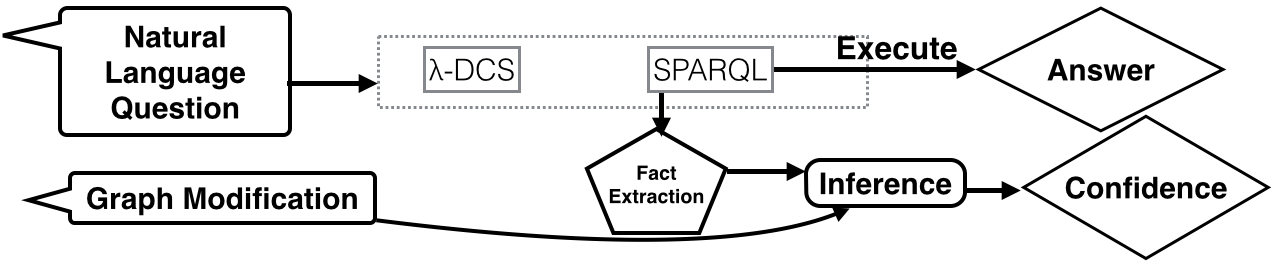
\includegraphics[width=0.9\linewidth]{images/probqa-pipeline.png}
 \caption{Probabilistic knowledge base assisted question answering demonstration pipeline.}
\label{fig:probqa-pipeline}
\end{figure*}


During the demo, attendees will be given the work flow shown in Figure~\ref{fig:probqa-pipeline}.
An attendee may provide a natural language question to the interface of retrieve one of the pre-seeded utterances.
This question is then translated to the \(\lambda\)-DCS and SPARQL using the SEMPRE system.
The user is then shows the answer to the question, as computed by the SPARQL
query and also the truthfulness result of the answer.

Alternatively, an attendee may interact with the knowledge base through a graphical interface.
Attendees will be able to search through the set of existing facts or use a graph to explore connections between graphs.
New probabilistic facts and rules can also be added to the system through the interface.
Users can also remove or alter the existing facts and rerun queries or answer more questions.
The status of queries and the underlying processes are displayed on the main interface.




%We can visualize the ranking of candidates with each candidates truthfulness value.

%Describe D3 visualization of graph and rule display
%Describe user interaction with graph
%Describe user selecting facts
%Describe users removing facts

%Features
%  Add the auto complete for previous questions.

%Describe how users will be able to alter parameters.


The demo application is developed using AngularJS\@ to be completely compatible with desktop and mobile devices.
We also loaded the data sets described in Section~\ref{sec:probqa-dataset} into a PostgreSQL DBMS\@.
We trained SEMPRE models for question answering on each of the three knowledge bases.
We translate the SPARQL queries to relational format using OpenRDF and Apache Jena SDB\@.
%Describe the tables 
%Describe the functions that are called
%Describe the parallelism
We install the database and web server on docker system container, so any modifications by demo can be quickly rolled back to the initial state.





